% !TeX spellcheck = en_US
%% 字体:方正静蕾简体
%%		 方正粗宋
\documentclass[a4paper,left=2.5cm,right=2.5cm,11pt]{article}
\usepackage[utf8]{inputenc}
\usepackage{fontspec}
\usepackage{cite}
\usepackage{xeCJK}
\usepackage{indentfirst}
\usepackage{titlesec}
\usepackage{longtable}
\usepackage{graphicx}
\usepackage{float}
\usepackage{rotating}
\usepackage{subfigure}
\usepackage{tabu}
\usepackage{amsmath}
\usepackage{setspace}
\usepackage{amsfonts}
\usepackage{appendix}
\usepackage{listings}
\usepackage{xcolor}
\usepackage{geometry}
\setcounter{secnumdepth}{4}
\usepackage{mhchem}
\usepackage{multirow}
\usepackage{extarrows}
\usepackage{hyperref}
\usepackage{caption}
\usepackage{color}

\titleformat*{\section}{\LARGE}
\renewcommand\refname{参考文献} %设置参考文献的形状
\renewcommand{\abstractname}{\sihao \cjkfzcs 摘{  }要}
%\titleformat{\chapter}{\centering\bfseries\huge\wryh}{}{0.7em}{}{}
%\titleformat{\section}{\LARGE\bf}{\thesection}{1em}{}{}
\titleformat{\subsection}{\Large\bfseries}{\thesubsection}{1em}{}{}
\titleformat{\subsubsection}{\large\bfseries}{\thesubsubsection}{1em}{}{}
\renewcommand{\contentsname}{{\cjkfzcs \centerline{目{  } 录}}}

\setCJKfamilyfont{cjkfzcs}{STSongti-SC-Regular}
% \setCJKfamilyfont{cjkhwxk}{STXingkai}
% \setCJKfamilyfont{cjkhwxk}{华文行楷}
% \setCJKfamilyfont{cjkfzcs}{方正粗宋简体}
\newcommand*{\cjkfzcs}{\CJKfamily{cjkfzcs}}
\newcommand*{\cjkhwxk}{\CJKfamily{cjkhwxk}}
% \newfontfamily\wryh{Microsoft YaHei}
% \newfontfamily\hwzs{STZhongsong}
\newfontfamily\hwst{STSong}
\newfontfamily\hwfs{STFangsong}
% \newfontfamily\jljt{MicrosoftYaHei}
% \newfontfamily\hwxk{STXingkai}
% \newfontfamily\hwzs{华文中宋}
% \newfontfamily\hwst{华文宋体}
% \newfontfamily\hwfs{华文仿宋}
% \newfontfamily\jljt{方正静蕾简体}
% \newfontfamily\hwxk{华文行楷}
\newcommand{\verylarge}{\fontsize{60pt}{\baselineskip}\selectfont}  
\newcommand{\chuhao}{\fontsize{44.9pt}{\baselineskip}\selectfont}  
\newcommand{\xiaochu}{\fontsize{38.5pt}{\baselineskip}\selectfont}  
\newcommand{\yihao}{\fontsize{27.8pt}{\baselineskip}\selectfont}  
\newcommand{\xiaoyi}{\fontsize{25.7pt}{\baselineskip}\selectfont}  
\newcommand{\erhao}{\fontsize{23.5pt}{\baselineskip}\selectfont}  
\newcommand{\xiaoerhao}{\fontsize{19.3pt}{\baselineskip}\selectfont} 
\newcommand{\sihao}{\fontsize{14pt}{\baselineskip}\selectfont}      % 字号设置  
\newcommand{\xiaosihao}{\fontsize{12pt}{\baselineskip}\selectfont}  % 字号设置  
\newcommand{\wuhao}{\fontsize{10.5pt}{\baselineskip}\selectfont}    % 字号设置  
\newcommand{\xiaowuhao}{\fontsize{9pt}{\baselineskip}\selectfont}   % 字号设置  
\newcommand{\liuhao}{\fontsize{7.875pt}{\baselineskip}\selectfont}  % 字号设置  
\newcommand{\qihao}{\fontsize{5.25pt}{\baselineskip}\selectfont}    % 字号设置 

\usepackage{diagbox}
\usepackage{multirow}
\boldmath
\XeTeXlinebreaklocale "zh"
\XeTeXlinebreakskip = 0pt plus 1pt minus 0.1pt
\definecolor{cred}{rgb}{0.8,0.8,0.8}
\definecolor{cgreen}{rgb}{0,0.3,0}
\definecolor{cpurple}{rgb}{0.5,0,0.35}
\definecolor{cdocblue}{rgb}{0,0,0.3}
\definecolor{cdark}{rgb}{0.95,1.0,1.0}
\lstset{   %设置代码的格式
	language=[x86masm]Assembler,
	numbers=left,
	numberstyle=\tiny\color{black},
	showspaces=false,
	showstringspaces=false,
	basicstyle=\scriptsize,
	keywordstyle=\color{purple},
	commentstyle=\itshape\color{cgreen},
	stringstyle=\color{blue},
	frame=lines,
	extendedchars=true, 
	xleftmargin=1em,
	xrightmargin=1em, 
	backgroundcolor=\color{cred},
	aboveskip=1em,
	breaklines=true,
	tabsize=4
} 

\newfontfamily{\monaco}{Monaco}
%\newfontfamily{\consolas}{Consolas}
%\setmonofont[Mapping={}]{Consolas}	%英文引号之类的正常显示,相当于设置英文字体
%\setsansfont{Consolas} %设置英文字体 Monaco, Consolas,  Fantasque Sans Mono
% \setCJKmainfont{华文中宋}
\setmainfont{Times New Roman}

\newcommand{\fic}[1]{\begin{figure}[H]
		\center
		\includegraphics[width=0.8\textwidth]{#1}
	\end{figure}}
	
\newcommand{\sizedfic}[2]{\begin{figure}[H]
		\center
		\includegraphics[width=#1\textwidth]{#2}
	\end{figure}}

\newcommand{\codefile}[1]{\lstinputlisting{#1}}


% 改变段间隔
\setlength{\parskip}{0.6em}
\linespread{1.1}
\usepackage{lastpage}
\usepackage{fancyhdr}
\pagestyle{fancy}

\lhead{\space \qquad \space}
\chead{homework4  \qquad Name:徐晓刚  \qquad Student ID:3140102480 \qquad}
\rhead{\qquad\thepage/\pageref{LastPage}}

\DeclareMathOperator\dif{d\!}


%设置双线页眉
\makeatletter                                         
\def\headrule{{\if@fancyplain\let\headrulewidth\plainheadrulewidth\fi%
		\hrule\@height 1.5pt \@width\headwidth\vskip1pt%上面线为1pt粗  
		\hrule\@height 0.5pt\@width\headwidth  %下面0.5pt粗            
		\vskip-2\headrulewidth\vskip-1.5pt}      %两条线的距离1pt      
	\renewcommand{\headrule}{\hrule depth0pt height0.15truemm width\textwidth}  
	\vspace{6mm}}     %双线与下面正文之间的垂直间距              
\makeatother  

\begin{document}
	
	%\clearpage
	%\thispagestyle{empty}
   \begin{longtable}{p{12cm}p{5cm}p{5cm}}
	%\begin{longtable}[位置]{列格式}
	%多行进行编写
	\multirow{6}{*}{ \xiaoerhao  \color{red}{Artificial intelligence}} \multirow{6}{*}{ \xiaoerhao Homework4 \space \space \space \space} & 专业:信息工程 \\
	& 姓名:徐晓刚 \\
	& 学院:信电学院 \\
	& 学号:3140102480 \\
	& 日期:\today \\
	& 地点:玉泉5舍 \\
\end{longtable}

\section*{Problem 1}
\subsection*{14.14}

\begin{itemize}
\item  \wuhao {\textbf{a.} For (i), we can see that B,I,M can influence each other so they will never be independent. For (ii), G is the only parent of J, so the network assert (ii). For (iii), G,B,I is the  Markov blanket of M, so the network assert (iii).}
\item \wuhao{\textbf{b.} According to the independent relation in the network, we can get the equation: \\ $P(b,i,\lnot m,g,j) = P(b)P(\lnot  m) P(i| b, \lnot m) P(g|b,i,\lnot m) P(j|g) = 0.2916$}
\item \wuhao{\textbf{c.} Since B,I,M are fixed true in the evidence we can treat G as having a prior of 0.9 : \\ $P(J |b,i,m) = \alpha \sum\limits_g P(J,g) = \alpha[P(J,g) + P(J,\lnot g)]\\ = <0.81,0.19>\\ $So the probability of going to jail is 0.81}
\item \wuhao {\textbf{d.}Intuitively, a person cannot be found guilty if not indicted, regardless of whether they
broke the law and regardless of the prosecutor. so G
is context-specifically independent of B and M given I = false.}
\item \wuhao {\textbf{e.} It's obvious that I and G
are parents of P . Because a pardon is more
likely if the person is actually innocent and if the prosecutor is politically motivated, so B and M as parents of P. The pardon may not be jailed,  so P is a parent of J. The new network can be see as following:\\
\begin{figure}[ht]
\centering
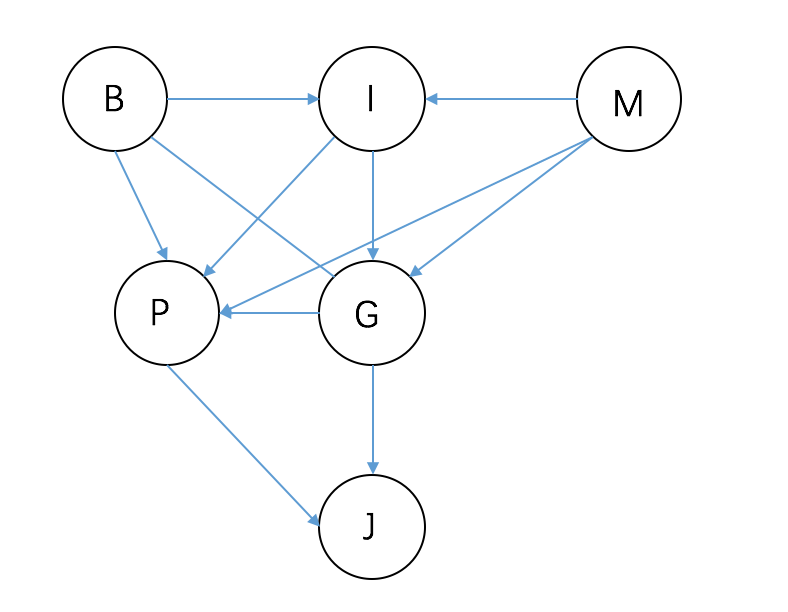
\includegraphics[width=10cm]{1.png}  
\caption*{\small\it The new network}
\end{figure} }
\end{itemize}

\section*{Problem 2}
\subsection*{14.15}
\begin{itemize}
\item \wuhao {\textbf{a.} $P(B|j,m) \\ = \alpha P(B) \sum\limits_e P(e) \sum\limits_a P(a|b,e) P(j|a)P(m|a) \\ = \alpha P(B)\sum\limits_e P(e) [0.9 \times 0.7 \times(\begin{pmatrix}
	0.95 & 0.29 \\ 0.94 & 0.001 \end{pmatrix}) + 0.05 \times 0.01 \times (\begin{pmatrix}
	0.05 & 0.71 \\ 0.06 & 0.999 \end{pmatrix}) ] \\ = \alpha P(B)\sum\limits_e P(e)  (\begin{pmatrix}
	0.598525 & 0.183055 \\ 0.59223 & 0.0011295 \end{pmatrix}) \\ = \alpha (\begin{pmatrix}
	0.001\\ 0.999 \end{pmatrix}) \times (\begin{pmatrix} 0.59224259\\ 0.001493351 \end{pmatrix}) \\= <0.284, 0.716>  $}
\item \wuhao {\textbf{b.} There are 7 additions, 16 multiplications, and 2 divisions. The enumeration algorithm has two extra multiplications. }
\item \wuhao {\textbf{c.} If we compute $P(X_1 | X_n = true)$ using enumeration, we have to evaluate two complete binary trees, each of depth n-1, so the tota work is $O(2^n)$.\\ If we use the method of variable elimination instead, the factors never grow beyond two variables. The total work is $O(n)$.}
\item \wuhao {\textbf{d.} Prove:\\
	First, based on the inductive hypothesis, we can assume that any polytree with n nodes can
be evaluated in time proportional to the size of the polytree . \\
	Next, consider a polytree with n + 1 nodes. To eliminate any leaf node, we have to do work proportional to the size of its CPT. Then, because the
network is a polytree, we are left with independent subproblems, one for each parent.
\\Each subproblem takes total work proportional to the sum of its CPT sizes, so the total
work for n + 1 nodes is proportional to the sum of CPT sizes}
\end{itemize}


\section*{Problem 3}
\subsection*{15.13}
We can see that there are three variables: \\ $S_t$, whether the student gets enough sleep; \\ $R_t$, whether they have red eyes in the class; \\ $C_t$, whether the student sleeps in class. It's obvious that $S_t$ is a parent of $S_{t+1}, R_t, C_t $  \\
The CPT are given as following:\\
$P(s_0) = 0.7 , P(s_{t+1}|s_t) = 0.8, P(s_{t+1}| \lnot s_t) = 0.3, \\
P(r_t|s_t) =0.2, P(r_t|\lnot s_t) = 0.7 ,\\ P(c_t|s_t) = 0.1, P(c_t|\lnot s_t)\\$
To reformulate as an HMM with a single observation node, simply combine the 2-valued variables “having red eyes” and “sleeping in class” into a single 4-valued variable. The Probability table are as following :

	\centering
	\begin{tabular}{|c|c|}
		\hline
		$S_0$ & $P(S_0)$\\
		\hline
		s & 0.7 \\
		\hline
		$\lnot s$ & 0.3\\
		\hline
	\end{tabular}
\\
    \begin{tabular}{|c|c|c|}
		\hline
		$R_t$ & $S_t$ & $P(R_t| S_t)$\\
		\hline
		r & s & 0.2 \\
		\hline
		$\lnot r$& s & 0.8\\
		\hline
		 r& $\lnot s $ & 0.7\\
		\hline
		$\lnot r$&$\lnot s$ & 0.3\\		
		\hline
	\end{tabular}
\begin{tabular}{|c|c|c|}
	\hline
	$S_{t+1}$ & $S_t$ & $P(S_{t+1}| S_t)$\\
	\hline
	$s_{t+1}$ & $s_t$ & 0.8 \\
	\hline
	$\lnot s_{t+1}$ & $s_t$ & 0.2\\
	\hline
	$s_{t+1}$& $\lnot s_t $ & 0.3\\
	\hline
	$\lnot s_{t+1}$& $\lnot s_t $& 0.7\\		
	\hline
\end{tabular}
\begin{tabular}{|c|c|c|}
	\hline
	$C_{t}$ & $S_t$ & $P(C_{t}| S_t)$\\
	\hline
	$c$ & $s$ & 0.1 \\
	\hline
	$\lnot c$ & $s$ & 0.9\\
	\hline
	$c$& $\lnot s $ & 0.3\\
	\hline
	$\lnot c$& $\lnot s $& 0.7\\		
	\hline
\end{tabular}\\
If we reformulate this model into HMM, we can set the observation as $O_t$
\begin{tabular}{|c|c|c|c|c|c|}
	\hline
	$O_{t}$ & $S_t$ & $P(O_{t}| S_t)$\\
	\hline
	$r,c$ & $s$ & 0.02 \\
	\hline
	$r,\lnot c$ & $s$ & 0.18\\
	\hline
	$\lnot r, c$ & $s$ & 0.08 \\
	\hline
	$\lnot r, \lnot c$ & $s$ & 0.72\\
	\hline
	$r,c$ & $\lnot s$ & 0.21 \\
	\hline
	$r,\lnot c$ & $\lnot  s$ & 0.49\\
	\hline
	$\lnot r, c$ & $\lnot s$ & 0.09 \\
	\hline
	$\lnot r, \lnot c$ & $\lnot s$ & 0.21\\
	\hline
\end{tabular}


\section*{Problem4}
\subsection*{a.}
\begin{tabular}{|c|c|}
	\hline
	$Y$ & $P(Y)$ \\
	\hline
	$-1$ & $0.5$\\
	\hline
	$+1$ & $0.5$\\
	\hline
\end{tabular}
\begin{tabular}{|c|c|c|}
	\hline
	$X_1$ & $P(X_1|Y=-1)$ &$P(X_1|Y=+1)$ \\
	\hline
	$0$ & $1/3$ & 2/3\\
	\hline
	$1$ & $2/3$ & 1/3\\
	\hline
\end{tabular}
\begin{tabular}{|c|c|c|}
	\hline
	$X_2$ & $P(X_2|Y=-1)$ &$P(X_2|Y=+1)$ \\
	\hline
	$0$ & $2/3$ & 2/3\\
	\hline
	$1$ & $1/3$ & 1/3\\
	\hline
\end{tabular}

\subsection*{b.}
In this problem we assume k = 1\\
\begin{tabular}{|c|c|}
	\hline
	$Y$ & $P(Y)$ \\
	\hline
	$-1$ & $0.5$\\
	\hline
	$+1$ & $0.5$\\
	\hline
\end{tabular}
\begin{tabular}{|c|c|c|}
	\hline
	$X_1$ & $P(X_1|Y=-1)$ &$P(X_1|Y=+1)$ \\
	\hline
	$0$ & $2/5$ & 3/5\\
	\hline
	$1$ & $3/5$ & 2/5\\
	\hline
\end{tabular}
\begin{tabular}{|c|c|c|}
	\hline
	$X_2$ & $P(X_2|Y=-1)$ &$P(X_2|Y=+1)$ \\
	\hline
	$0$ & $3/5$ & 3/5\\
	\hline
	$1$ & $2/5$ & 2/5\\
	\hline
\end{tabular}


\subsection*{c.}
$P(Y, X_1 = 0, X_2 = 0) $ \\= $ \begin{pmatrix} P(Y=+1)\times P(X_1=0|Y=+1)\times P(X_2 =0|Y=+1)\\  P(Y=-1)\times P(X_1=0|Y=-1)\times P(X_2 =0|Y=-1)\end{pmatrix}  $  $=\begin{pmatrix} 0.18\\ 0.12  \end{pmatrix}$
\\ $P(X_1 = 0, X_2 = 0) = \frac{2+1}{6+4}  =0.3$
\\ $P(Y|X_1=0,X_2=0) = <0.6, 0.4>$
\subsection*{d.}
As $k \rightarrow \infty $\\
$P(Y, X_1 = 0, X_2 = 0)  = \begin{pmatrix} 1/8\\ 1/8  \end{pmatrix}$\\
$P(X_1 = 0, X_2 = 0) = \frac{2+k}{6+4k}  =1/4$
\\ $P(Y|X_1=0,X_2=0) = <0.5, 0.5>$
\subsection*{e.}
The sets that would enable a linear binary classifier include (v),(viii)

\section*{Problem5}
\begin{flushleft}   We first draw the four examples using axes x1, x2, denoting class by +/-. \\
Label them (p1, ..., p4) .\\
we will set a transformation that will make these points linearly separable:\\
\end{flushleft}
$y_1 = x_1 $, \\$ y_2 = (x_1-x_2)^2$
\\\begin{flushleft}  The margin is 2. For the transformation above, the max-margin separator is at y2 = 2. \\We get the separating line :\\ \end{flushleft}
$x_1 - x_2 = \sqrt{2}$ or $x_1 - x_2 = -\sqrt{2}$

\begin{figure}[ht]
	\centering
	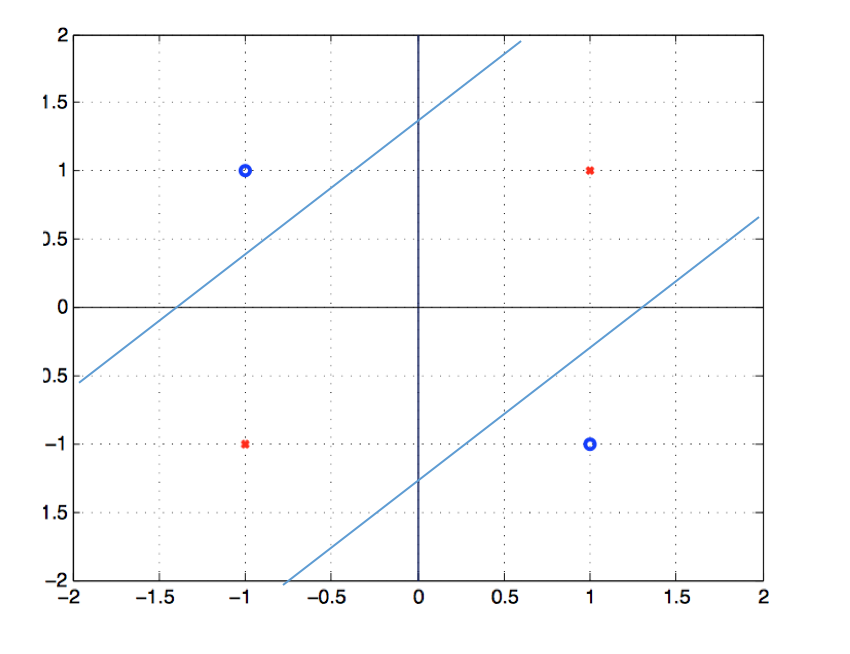
\includegraphics[width=10cm]{2.png}  
\end{figure}

%\begin{figure}[ht]
%\centering
%\includegraphics[width=10cm]{pic3.png}  
%\caption*{\small\it Figure 10.4: 4个可能信息以及二值编码的例子}
%\end{figure}

%\begin{itemize}
%\item  \wuhao %{\color{red}{为了传送概率密度函数为$Pr(z)$的随机变量$z$,我们需要$-log_2Pr(z)$位信息}} %\par
%\end{itemize}

%\begin{quote}
%\centering {\color{red}{$length=constant + log\sigma + \frac{(y-\theta)^2}{\sigma^2} + %\frac{\theta^2}{2} \qquad(7.45)$}}
%\end{quote}

\end{document}

